\section{Lab 4 - Finite-State Machines}

\subsection{Introduction}
A \emph{finite-state machine} (FSM) is a model for sequential logic that consists of a set of states (including an initial or reset state) a set of inputs/outputs and a transition function that shows the transition from one state to other states. The state the FSM is in at any given time is called the {\it current} state. The FSM can change from one state to another when initiated by a triggering event or condition (input); this is called a transition. This lab will examine a simple FSM to give the general idea of how they work, and build upon it to create a system modeled off of a real world example, a vending machine.

\subsection{Pre-lab}

Before coming to the lab, please complete the following activity and upload the results to Sakai.
\begin{itemize}
	\item By examining the code in Listing \ref{code:fsm} write out its state machine transition graph.
\end{itemize}


\subsection{Lab Activities}

\subsubsection{FSM}

Given the state machine transition graph in Figure \ref{fig:fsm}, design VHDL code for the state transitions of this diagram. Note that in the state transition graph, we show the transition behavior as input/output where the input is denoted as D$_1$D$_0$ and the output is denoted as  Z$_1$Z$_0$. For example 00/01 means D$_1$D$_0$ = 00 and causes  Z$_1$Z$_0$ = 01. Assume that state A is the reset state for this machine.

\begin{figure}[H]
	\centering
	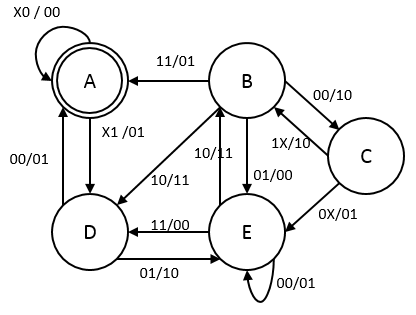
\includegraphics[width=100mm]{Lab4/figures/fsm.png}
	\caption{State machine transition graph}
	\label{fig:fsm}
\end{figure}

The code below shows a simple example of a FSM. You can build upon this code in completing this lab. 

\begin{lstlisting}[caption=Sample code for a Finite State Machine, label=code:fsm]
-- User-Encoded State Machine
library ieee;
use ieee.std_logic_1164.all;

entity state_machine is
	port(clk	 	 : in std_logic;
		reset	  : in std_logic;
		input	  : in std_logic;
		output	  : out std_logic);
	
end entity;

architecture rtl of state_machine is
	-- Build an enumerated type for the state machine
	type count_state is (A, B, C, D);
	
	-- Registers to hold the current state and the next state
	signal present_state, next_state	   : count_state;
	
	-- Attribute to declare a specific encoding for the states
	attribute syn_encoding				  : string;
	attribute syn_encoding of count_state : type is "11 01 10 00";
	
begin
	-- Move to the next state
	process(clk, reset)
	begin
		if reset = '1' then
			present_state <= A;
		elsif (rising_edge(clk)) then
			present_state <= next_state;
		end if;
	end process;

	-- Determine what the next state will be, and set the output bits
	process (present_state, input)
	begin
		case present_state is
			when A =>
				if (input = '0') then
					next_state <= B;
					output <= '0';
				else
					next_state <= D;
					output <= '0';
				end if;
			when B =>
				if (input = '0') then
					next_state <= C;
					output <= '1';
				else
					next_state <= A;
					output <= '0';
				end if;
			when C =>
				if (input = '0') then
					next_state <= D;
					output <= '0';
				else
					next_state <= B;
					output <= '1';
				end if;
			when D =>
				if (input = '0') then
					next_state <= A;
					output <= '0';
				else
					next_state <= C;
					output <= '1';
				end if;
		end case;
	end process;
	
end rtl;
\end{lstlisting}

\subsubsection{Vending Machine}

Design a custom finite-state machine to control a vending machine to dispense products. The design has the following specifications:

\begin{enumerate} 

	\item The state machine should have three states:

	\begin{itemize}
		\item \emph{IDLE}: This is the default (reset) state for the machine. The machine should stay in this state until at least one product is selected. Being that this is the reset state, you should initialize the signals QUARTERS, COST, and DISPENSE\_READY to zero. Make sure that LEDR0 to LEDR17 along with LEDG1 to LED8 are set to off. While in this state, you should display a dash across all HEX displays. 

		\item \emph{PRODUCT\_SELECT}: The state machine will move into this state if product(s) are selected through use of the switches (SW0 - SW15) on the FPGA board. Display the total cost in number of quarters needed of all products selected on HEX5 - HEX4 in hexadecimal.  KEY3 and KEY2 should increment QUARTERS by a dollar and quarter respectively when pressed. Display the value of QUARTERS on HEX1 - HEX0. When the correct number of quarters have been inserted, the signal DISPENSE\_READY should go HIGH (which should be shown on LEDG8) and the state should transition to DISPENSE. A list of available products and their cost can be found in Table \ref{tab:costlist}.

		\item \emph{DISPENSE}: Once the proper amount of quarters have been deposited, the item should be dispensed from the machine. To show that the item(s) have been dispensed, turn on LEDR0-LEDR17 and set the next state to idle.

	\end{itemize}
	
	\item KEY0 will act as a CLOCK input and KEY1 will act as a coin return or rest. The states should transition on the rising edge. This means that you should select a product and then send a CLOCK pulse to calculate the cost of the item(s) selected. Then add quarters into the machine and send another CLOCK pulse when there is the right amount of quarters. If there is not enough quarters inserted, the state should not change. Once the item(s) are dispensed, send another CLOCK pulse to return to IDLE.

	\item The current state; \emph{IDLE}, \emph{PRODUCT\_SELECT}, and \emph{DISPENSE} should be displayed by turning on LEDG0 - LEDG2 respectively.
	
	\item Both signals QUARTERS and COST should be of the type INTEGER with a range of 0 to 40.  You will need to use the package \emph{ieee.numeric_std.all}.
	
\end{enumerate}

\begin{table}[H]
	\centering
	\caption{List of vending machine items, cost, and switch correspondence}
	\begin{tabular}{ | c | c | c | }
		\hline                        
 		\bf Product & \bf Cost & \bf Switch\\ \hline
 		SODA\_CAN[0:3] & \$1.00 & SW12 - SW15 \\ \hline
		CHIPS[0:3] & \$0.75 & SW8 - SW11 \\ \hline
		CHOCOLATE[0:3] & \$0.50 & SW4 - SW7 \\ \hline
		BUBBLE\_GUM[0:3] & \$0.25 & SW0 - SW3 \\
 		\hline
	\end{tabular}
	\label{tab:costlist}
\end{table}


\subsection{Lab Report}

After completing the activities in this lab you should create a zip folder with the following and then submit it to Sakai:

\begin{itemize}
	\item Commented VHDL code.
	\item VHDL test bench for the FSM activity.
	\item Waveform for the FSM activity.
	\item Pictures of the results from the vending machine activity.
	\item A discussion on the results of compilation including longest path delay, the total number of logic elements used, and issues you encountered while performing the lab.
\end{itemize}


